%==============================================================================
% Re-examining Knowledge-Graph Augmentation for Zero-Shot Drug Repurposing
% A Scaled Reproduction and Ablation of TxGNN
%
% IEEE conference format. Compile with pdflatex (run twice):
%     pdflatex final_report.tex ; pdflatex final_report.tex
% Figures (real data plots) are in ./figures/ ; IEEEtran.cls is bundled.
%==============================================================================
\documentclass[conference]{IEEEtran}

\usepackage{cite}
\usepackage{graphicx}
\usepackage[table,dvipsnames]{xcolor}
\usepackage{booktabs}
\usepackage{array}
\usepackage{amsmath,amssymb}
\usepackage{url}
\usepackage{sectsty}
\usepackage[hidelinks]{hyperref}

%--- brand palette ------------------------------------------------------------
\definecolor{brandnavy}{HTML}{16223B}
\definecolor{brandindigo}{HTML}{4F46E5}
\definecolor{brandteal}{HTML}{0EA5A4}
\definecolor{rowalt}{HTML}{EEF2F8}
\definecolor{cgood}{HTML}{16A34A}
\definecolor{cbad}{HTML}{E0563B}

\sectionfont{\color{brandnavy}}
\subsectionfont{\color{brandindigo}}

\hypersetup{colorlinks=true, linkcolor=brandindigo, citecolor=brandteal, urlcolor=brandindigo}

\newcommand{\hdr}[1]{\textcolor{white}{\textbf{#1}}}
\newcommand{\best}[1]{\textcolor{cgood}{\textbf{#1}}}
\newcommand{\worse}[1]{\textcolor{cbad}{#1}}

%--- REPLACE WITH YOUR DEPLOYED SITE URL --------------------------------------
\newcommand{\projecturl}{https://kg-repurposing-study.vercel.app}

\begin{document}

\title{Re-examining Knowledge-Graph Augmentation for\\
Zero-Shot Drug Repurposing:\\
A Scaled Reproduction and Ablation of TxGNN}

\author{
\IEEEauthorblockN{Khairullah Ibrahim Khail}
\IEEEauthorblockA{
Supervisor: Dr.~Ishaq\\
Department of Computer Science\\
Email: \texttt{ibrahimkhil975@gmail.com}}
}

\maketitle

%==============================================================================
\begin{abstract}
Drug repurposing offers a faster route to therapy, but most computational
methods need labelled drug--disease pairs that do not exist for rare diseases.
TxGNN addresses this with a heterogeneous knowledge graph (PrimeKG) and a
disease-similarity module that enables zero-shot prediction. We reproduce TxGNN
at reduced scale on a single 8\,GB GPU ($\texttt{hidden\_dim}=64$ vs.\ the
published $512$) and use it to answer six pre-registered questions about whether,
and how much, the knowledge graph (KG) actually helps. All metrics are computed
from result files over seeds $[42,0,1]$; none are entered by hand. We find that
(i) on the standard split a no-message-passing baseline \emph{beats} the KG model
on indication AUPRC ($0.893$ vs.\ $0.825$); (ii) two-phase training remains the
strongest and fastest recipe for zero-shot indication ($0.736$); (iii) zero-shot
prediction is a necessity because ${\sim}92\%$ of diseases carry no indication
label; and (iv) contrary to the common assumption, the attention mechanism is
not merely optional but \emph{detrimental}---removing it raises zero-shot
indication AUPRC to $0.772$ ($\Delta=-0.036$) while running ${\sim}22\times$
faster. Findings are scoped to the reduced-scale setting and reported as
observed, including null and negative results.
\end{abstract}

\begin{IEEEkeywords}
drug repurposing, knowledge graph, graph neural network, zero-shot learning,
TxGNN, PrimeKG, ablation study.
\end{IEEEkeywords}

%==============================================================================
\section{Introduction}
Repurposing an approved drug for a new indication is cheaper and faster than
\emph{de novo} development, but candidate-based models require labelled
drug--disease pairs, and for the long tail of rare diseases those labels are
absent. TxGNN~\cite{huang2024} reframes the task around a heterogeneous knowledge
graph, PrimeKG~\cite{chandak2023}, and a disease-similarity module that transfers
evidence from well-studied diseases to unseen ones, enabling \emph{zero-shot}
prediction.

This work is a \emph{scaled reproduction}: an 8\,GB RTX~4060 forces
$\texttt{hidden\_dim}=64$ instead of the published $512$, so every result is
labelled \texttt{scaled\_reproduction} and is never merged with the paper's
figures. The aim is not to beat the published model but to test, under a fixed
and audited protocol, which of its components are actually responsible for its
behaviour.

\subsection{A Note on Model Class}
The TxGNN encoder is a Heterogeneous Graph Transformer (HGT); the word
``Transformer'' names its multi-head attention aggregation. It is a
\textbf{graph neural network}, not a language model, and no language model is
trained here. We therefore restate the informal question ``do Transformers/LLMs
do better with a KG?'' as: \emph{does a GNN that message-passes over a KG beat
one that does not?} Text--graph hybrids such as KG-BERT~\cite{kgbert2019} and
DRAGON~\cite{dragon2022} are noted as background only; they target different
datasets and are not evaluated here.

\subsection{Research Questions}
\begin{enumerate}
\item Does KG message passing beat a no-KG baseline?
\item Is there a better recipe than TxGNN's two-phase training?
\item Why is zero-shot prediction preferred?
\item What do two case studies (one rare, one common) reveal?
\item How does a plain GNN compare to TxGNN (tabular)?
\item Is the attention mechanism optional?
\end{enumerate}

%==============================================================================
\section{Methods}
\subsection{Data and Splits}
PrimeKG~\cite{chandak2023} (Harvard Dataverse, CC0) provides $8{,}100{,}498$
edges over $129{,}375$ nodes and $10$ node types; therapeutic edges total
$18{,}776$ indications and $61{,}350$ contraindications. We build two regimes for
seeds $[42,0,1]$: a \emph{standard} random edge hold-out, and a \emph{zero-shot}
split in which $641$ held-out diseases keep no treatment edge in training. A
leakage audit confirms zero leaking diseases for every seed before any zero-shot
result is accepted. Two oversized relations
(\texttt{anatomy\_protein\_present}, \texttt{drug\_drug}) are excluded from
message passing for VRAM reasons, leaving ${\sim}2.4$M of $8.1$M edges.

\subsection{Models}
The plain GNN is a two-layer HGT with a learnable embedding table per node type
and dot-product scoring; setting depth$=0$ disables message passing (the no-KG
control). The scaled TxGNN adds a disease-affinity head (cosine projection,
$k=5$ support diseases) and a triplet metric loss, trained in two phases
(self-supervised KG pretraining, then therapeutic fine-tuning). Two Q2
alternatives---single-stage multi-task and joint InfoNCE contrastive---collapse
the two phases. Q6 toggles attention (HGT vs.\ mean aggregation) and the
affinity head.

\subsection{Evaluation}
The primary metric is AUPRC, secondary AUROC, with random negatives at $1{:}5$
for all cross-model (flat) comparisons and per-disease full ranking for the
zero-shot degradation analysis. Results are reported as mean~$\pm$~std over seeds
$[42,0,1]$ and computed directly from the result files.

%==============================================================================
\section{Results}

\subsection{Q1: KG Augmentation vs.\ No-KG}
Message passing does not lift indication AUPRC on either split
(Table~\ref{tab:q1}, Fig.~\ref{fig:q1}). On the standard split the no-KG model is
clearly ahead; on zero-shot, indication is a statistical wash and the KG model
only helps contraindication. We report this null result as observed.

\begin{table}[t]
\centering
\caption{Q1 --- Plain GNN with vs.\ without KG message passing (AUPRC).}
\label{tab:q1}
\renewcommand{\arraystretch}{1.25}
\begin{tabular}{l l c c}
\rowcolor{brandindigo}
\hdr{Model} & \hdr{Split} & \hdr{AUPRC ind} & \hdr{AUPRC contra}\\
\texttt{gnn\_no\_kg} & standard  & \best{0.893\,$\pm$\,0.006} & \best{0.945\,$\pm$\,0.002}\\
\rowcolor{rowalt}
\texttt{gnn\_kg}     & standard  & 0.825\,$\pm$\,0.022 & 0.895\,$\pm$\,0.026\\
\texttt{gnn\_no\_kg} & zero-shot & 0.704\,$\pm$\,0.027 & 0.725\,$\pm$\,0.008\\
\rowcolor{rowalt}
\texttt{gnn\_kg}     & zero-shot & \best{0.714\,$\pm$\,0.026} & \best{0.831\,$\pm$\,0.016}\\
\end{tabular}
\end{table}

\begin{figure}[t]
\centering
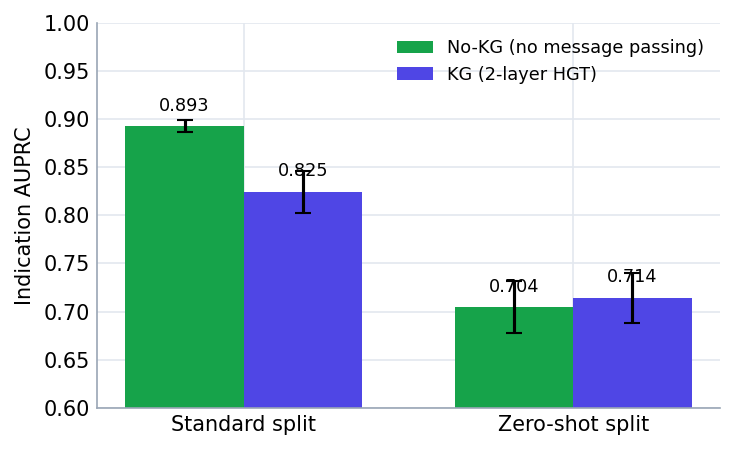
\includegraphics[width=\columnwidth]{figures/fig_q1.png}
\caption{Q1: indication AUPRC of the no-KG control vs.\ the KG model, per split
(mean over seeds $[42,0,1]$; error bars = std). Message passing does not help.}
\label{fig:q1}
\end{figure}

\subsection{Q2: Is Two-Phase Training Beatable?}
Under the pre-registered criterion (higher zero-shot indication AUPRC at
equal-or-lower compute), neither alternative beats two-phase training, which is
also the fastest on zero-shot (Table~\ref{tab:q2}, Fig.~\ref{fig:q2}).

\begin{table}[t]
\centering
\caption{Q2 --- Two-phase vs.\ alternatives (AUPRC; wall-clock in seconds).}
\label{tab:q2}
\renewcommand{\arraystretch}{1.25}
\begin{tabular}{l l c c c}
\rowcolor{brandindigo}
\hdr{Method} & \hdr{Split} & \hdr{ind} & \hdr{contra} & \hdr{Wall}\\
\texttt{txgnn\_two\_phase}   & zero-shot & \best{0.736} & 0.832 & \best{71.6}\\
\rowcolor{rowalt}
\texttt{single\_stage}       & zero-shot & 0.706 & 0.833 & 130.7\\
\texttt{joint\_contrastive}  & zero-shot & \worse{0.670} & \best{0.854} & 97.1\\
\rowcolor{rowalt}
\texttt{txgnn\_two\_phase}   & standard  & 0.816 & 0.899 & 183.8\\
\texttt{single\_stage}       & standard  & 0.723 & 0.863 & 100.3\\
\rowcolor{rowalt}
\texttt{joint\_contrastive}  & standard  & 0.739 & 0.862 & 95.9\\
\end{tabular}
\end{table}

\begin{figure}[t]
\centering
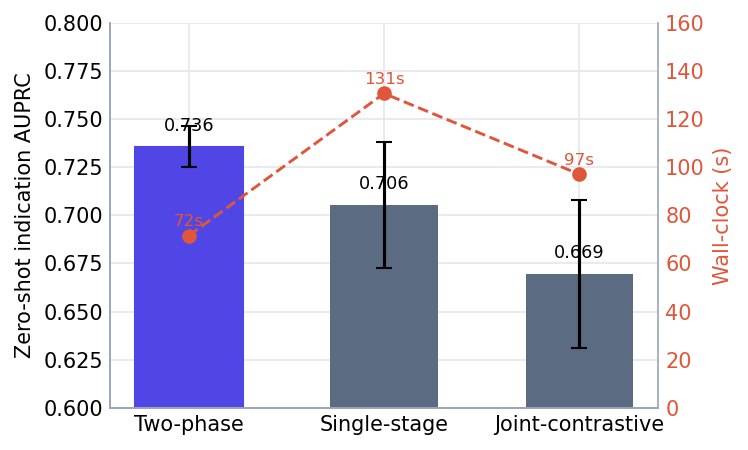
\includegraphics[width=\columnwidth]{figures/fig_q2.png}
\caption{Q2: zero-shot indication AUPRC (bars, left axis) and wall-clock time
(dashed, right axis) for the three training recipes. Two-phase is both the most
accurate and the fastest.}
\label{fig:q2}
\end{figure}

\subsection{Q3: Why Zero-Shot?}
About $92\%$ of PrimeKG diseases have no indication edge, so a supervised
classifier has no labels for them. The degradation curve
(Fig.~\ref{fig:degradation}) shows standard-split AUPRC collapsing as training
edges vanish, while the zero-shot TxGNN holds ${\sim}0.74$ across all held-out
diseases---zero-shot is a necessity, not a preference.

\begin{figure}[t]
\centering
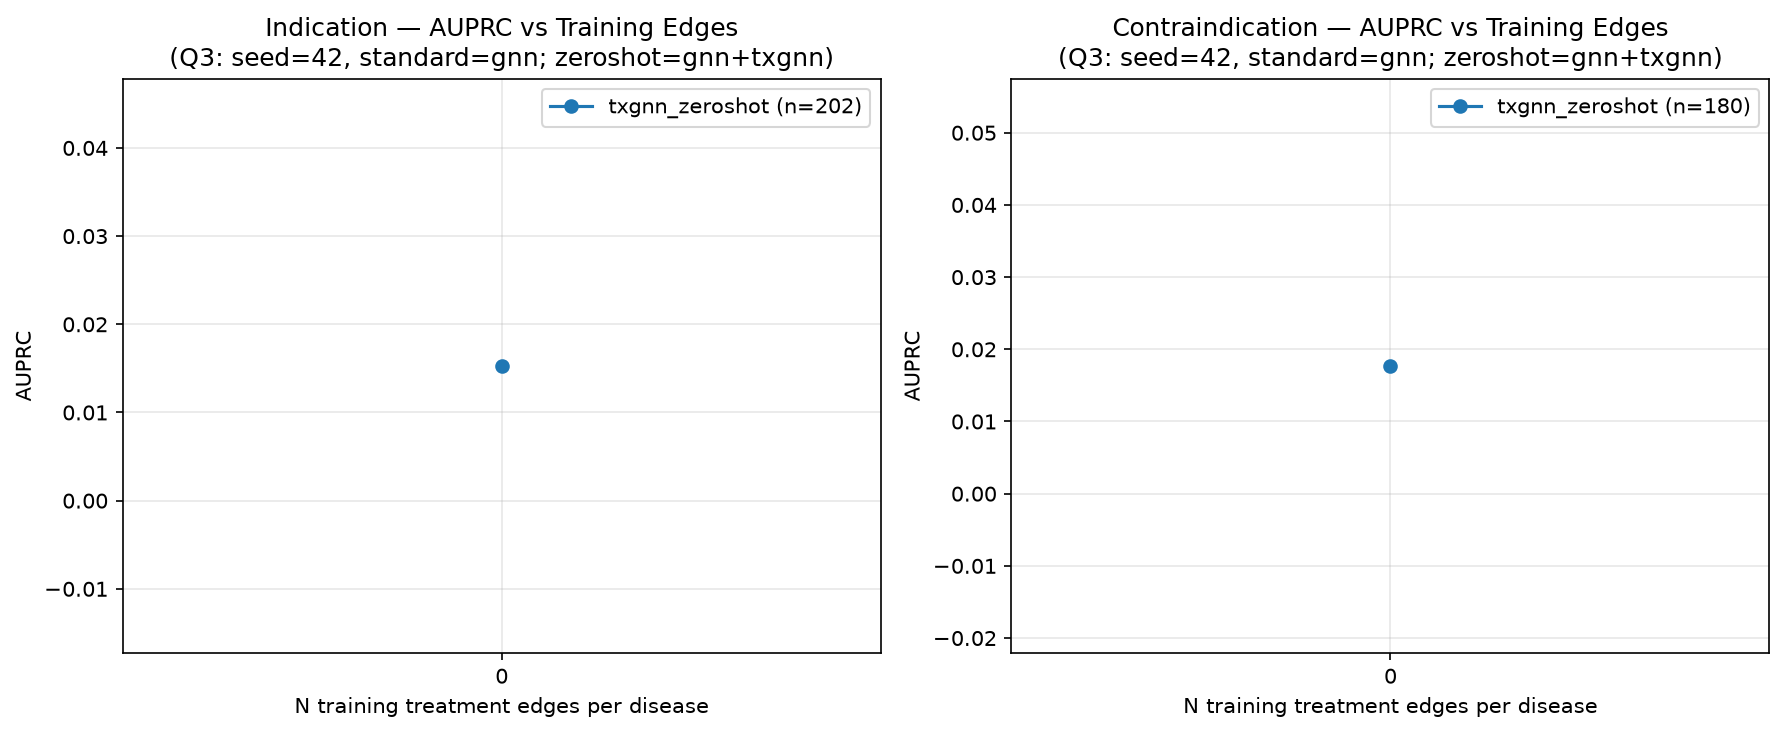
\includegraphics[width=\columnwidth]{figures/fig_degradation.png}
\caption{Q3 degradation curve: per-disease AUPRC vs.\ the number of training
treatment edges (seed 42), binned. Performance collapses toward the zero-edge
regime that the zero-shot model is designed for.}
\label{fig:degradation}
\end{figure}

\subsection{Q5: GNN vs.\ TxGNN}
Table~\ref{tab:q5} reports the full comparison. The simplest model wins the
standard split; TxGNN's advantage appears only on zero-shot, and only by
${\sim}3.2$ points over the no-KG baseline. Published figures from
Huang \emph{et al.}~\cite{huang2024} are shown in separate columns and never
merged with ours.

\begin{table*}[t]
\centering
\caption{Q5 --- Full comparison (AUPRC, mean\,$\pm$\,std). Paper figures from
Huang \emph{et al.}~\cite{huang2024}, Suppl.\ Tables S1/S2; ``---'' = not
applicable / not run.}
\label{tab:q5}
\renewcommand{\arraystretch}{1.25}
\begin{tabular}{l l c c c c c}
\rowcolor{brandindigo}
\hdr{Model} & \hdr{Split} & \hdr{ind (scaled)} & \hdr{ind (paper)} &
\hdr{contra (scaled)} & \hdr{contra (paper)} & \hdr{Wall (s)}\\
\texttt{gnn\_no\_kg}        & standard  & \best{0.893\,$\pm$\,0.006} & --- & 0.945\,$\pm$\,0.002 & --- & 0.7\\
\rowcolor{rowalt}
\texttt{gnn\_kg}            & standard  & 0.825\,$\pm$\,0.022 & --- & 0.895\,$\pm$\,0.026 & --- & 145.5\\
\texttt{txgnn\_two\_phase}  & standard  & 0.816\,$\pm$\,0.012 & 0.91\,$\pm$\,0.02 & 0.899\,$\pm$\,0.010 & 0.82\,$\pm$\,0.01 & 183.8\\
\rowcolor{rowalt}
\texttt{single\_stage}      & standard  & 0.723\,$\pm$\,0.005 & --- & 0.863\,$\pm$\,0.012 & --- & 100.3\\
\texttt{joint\_contrastive} & standard  & 0.739\,$\pm$\,0.019 & --- & 0.862\,$\pm$\,0.014 & --- & 95.9\\
\rowcolor{rowalt}
\texttt{gnn\_no\_kg}        & zero-shot & 0.704\,$\pm$\,0.027 & --- & 0.725\,$\pm$\,0.008 & --- & 0.2\\
\texttt{gnn\_kg}            & zero-shot & 0.714\,$\pm$\,0.026 & --- & 0.831\,$\pm$\,0.016 & --- & 71.3\\
\rowcolor{rowalt}
\texttt{txgnn\_two\_phase}  & zero-shot & \best{0.736\,$\pm$\,0.011} & 0.90\,$\pm$\,0.02 & 0.832\,$\pm$\,0.010 & 0.80\,$\pm$\,0.01 & 71.6\\
\texttt{single\_stage}      & zero-shot & 0.706\,$\pm$\,0.033 & --- & 0.833\,$\pm$\,0.019 & --- & 130.7\\
\rowcolor{rowalt}
\texttt{joint\_contrastive} & zero-shot & 0.670\,$\pm$\,0.038 & --- & \best{0.854\,$\pm$\,0.016} & --- & 97.1\\
\end{tabular}
\end{table*}

\subsection{Q6: Is Attention Optional?}
The decision rule was fixed before running:
$\Delta = \text{AUPRC}_{\text{on}} - \text{AUPRC}_{\text{off}}$ on zero-shot
indication; $|\Delta| < 0.02$ means optional, $\Delta \le -0.02$ means harmful.
We measure $\Delta = 0.736 - 0.772 = \mathbf{-0.036}$: attention is
\textbf{detrimental} (Table~\ref{tab:q6}, Fig.~\ref{fig:q6}), and removing it runs
${\sim}22\times$ faster. This converges with the published model, which replaced
learnable attention with fixed degree-based gating. The affinity head, by
contrast, is beneficial: removing it drops AUPRC to $0.726$.

\begin{table}[t]
\centering
\caption{Q6 --- Attention/affinity ablation on the zero-shot split (AUPRC).}
\label{tab:q6}
\renewcommand{\arraystretch}{1.25}
\begin{tabular}{l c c c}
\rowcolor{brandindigo}
\hdr{Variant} & \hdr{ind} & \hdr{contra} & \hdr{Wall}\\
\texttt{txgnn} (attn,sim)       & 0.736 & \best{0.832} & 71.6\\
\rowcolor{rowalt}
\texttt{txgnn\_no\_attn}        & \best{0.772} & 0.787 & \best{3.2}\\
\texttt{txgnn\_no\_sim}         & 0.726 & 0.824 & ---\\
\rowcolor{rowalt}
\texttt{txgnn\_no\_both}        & 0.762 & 0.780 & ---\\
\end{tabular}
\end{table}

\begin{figure}[t]
\centering
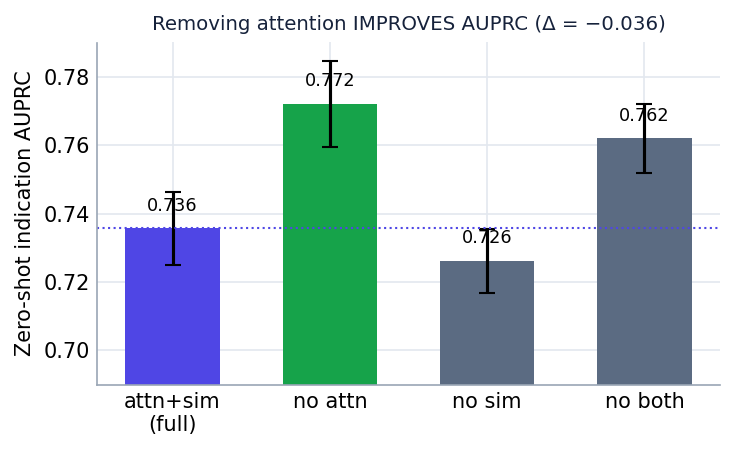
\includegraphics[width=\columnwidth]{figures/fig_q6.png}
\caption{Q6: zero-shot indication AUPRC for the four ablation variants
(error bars = std; dotted line = full model). Removing attention (green) gives
the best score.}
\label{fig:q6}
\end{figure}

%==============================================================================
\section{Case Studies (Q4)}
Two diseases were fixed before any prediction was inspected. For \emph{Familial
Hypertrophic Cardiomyopathy} (FHC, $n_{\text{pos}}=1$) the model fails: the one
known indication (Propranolol) is absent from the top-20 and per-disease AUPRC is
$0.025$ (Table~\ref{tab:caseA}). For \emph{Staphylococcus aureus infection}
($n_{\text{pos}}=45$) it is a partial success---Benzylpenicillin appears at
rank~18 and Mupirocin/Doxycycline are clinically plausible---though three
antineoplastics intrude into the top-10. In both cases the reasoning path runs
through disease--disease similarity, consistent with the Q6 finding that the
affinity head, not attention, carries the model.

\begin{table}[t]
\centering
\caption{Case A --- top-10 indication predictions for FHC (seed 42). None are
positive; per-disease AUPRC $=0.025$.}
\label{tab:caseA}
\renewcommand{\arraystretch}{1.2}
\begin{tabular}{c l c c}
\rowcolor{brandindigo}
\hdr{Rank} & \hdr{Drug} & \hdr{DrugBank} & \hdr{Score}\\
1  & Lutetium Lu 177 dotatate & DB13985 & $-1.038$\\
\rowcolor{rowalt}
2  & Lactose       & DB04465 & $-1.206$\\
3  & Emapalumab    & DB14724 & $-1.226$\\
\rowcolor{rowalt}
4  & Cysteine      & DB00151 & $-1.234$\\
5  & Sulfapyridine & DB00891 & $-1.251$\\
\rowcolor{rowalt}
6  & Etoposide     & DB00773 & $-1.263$\\
7  & Oleandomycin  & DB11442 & $-1.265$\\
\rowcolor{rowalt}
8  & Etretinate    & DB00926 & $-1.268$\\
9  & Quinacrine    & DB01103 & $-1.283$\\
\rowcolor{rowalt}
10 & Umifenovir    & DB13609 & $-1.293$\\
\end{tabular}
\end{table}

%==============================================================================
\section{Discussion and Conclusion}

\subsection{Scaled Findings vs.\ the Published Claim}
The published TxGNN reports a clear advantage from KG-based zero-shot transfer:
indication AUPRC of $0.90\pm0.02$ (zero-shot) and $0.91\pm0.02$ (standard), well
above the GNN baselines (Table~\ref{tab:q5}, paper columns)~\cite{huang2024}. Our
reduced-scale reproduction does \emph{not} recover that advantage. At
$\texttt{hidden\_dim}=64$ the no-message-passing baseline actually wins the
standard split ($0.893$ vs.\ $0.825$), and TxGNN's zero-shot edge over the no-KG
model shrinks to ${\sim}3.2$ points. This is a contrast of \emph{scale}, not a
refutation: three compounding reductions---embedding width $512\!\to\!64$, layers
$3\!\to\!2$, and learnable embeddings instead of the paper's pre-trained node
features---together with the VRAM-driven edge filtering remove most of the
capacity the full model needs to exploit KG structure. The attention result,
however, points the \emph{same} way at both scales: our ablation finds learnable
attention harmful, and the published model likewise discarded it in favour of a
fixed degree-based gate. The practical message is that KG augmentation and
disease-similarity transfer are genuinely useful at full scale, but their benefit
is capacity-dependent and can vanish---or reverse---once the model is shrunk to
commodity hardware. Any claim that ``the knowledge graph helps'' must therefore
be qualified by the model size at which it was measured.

\subsection{Summary and Outlook}
At this scale, KG message passing does not consistently help; two-phase training
is the best zero-shot recipe; zero-shot prediction is forced by label sparsity;
and the attention mechanism is harmful rather than merely optional. These results
are scoped to the reduced-scale setting ($\texttt{hidden\_dim}=64$, two layers,
filtered edges, seeds $[42,0,1]$) and are not claims about the full published
model; the $8\times$ reduction in embedding width is the most likely driver of
the gaps to the paper's figures. The case studies show the model leaning on
disease similarity, which explains both its zero-shot ability and its noisy
rankings for poorly-connected diseases. Future work should restore the published
width on larger hardware and re-test Q1 and Q6 there.

\smallskip
\noindent\textbf{Data and code availability.} All result files, splits, and the
figure-generation scripts used in this report are released with the project; a
browsable summary is hosted at \url{\projecturl}.

%==============================================================================
\begin{thebibliography}{1}
\bibitem{huang2024}
K.~Huang \emph{et al.}, ``A foundation model for clinician-centered drug
repurposing,'' \emph{Nature Medicine}, 2024, doi:10.1038/s41591-024-03233-x.

\bibitem{chandak2023}
P.~Chandak, K.~Huang, and M.~Zitnik, ``Building a knowledge graph to enable
precision medicine,'' \emph{Scientific Data}, vol.~10, no.~67, 2023.

\bibitem{kgbert2019}
L.~Yao, C.~Mao, and Y.~Luo, ``KG-BERT: BERT for knowledge graph completion,''
\emph{arXiv:1909.03193}, 2019.

\bibitem{dragon2022}
M.~Yasunaga \emph{et al.}, ``Deep bidirectional language-knowledge graph
pretraining,'' in \emph{Proc.\ NeurIPS}, 2022.
\end{thebibliography}

\end{document}
